\documentclass[tikz,border=5pt]{standalone}
\usepackage{amsmath}
\usetikzlibrary{arrows.meta,positioning,calc}

\begin{document}
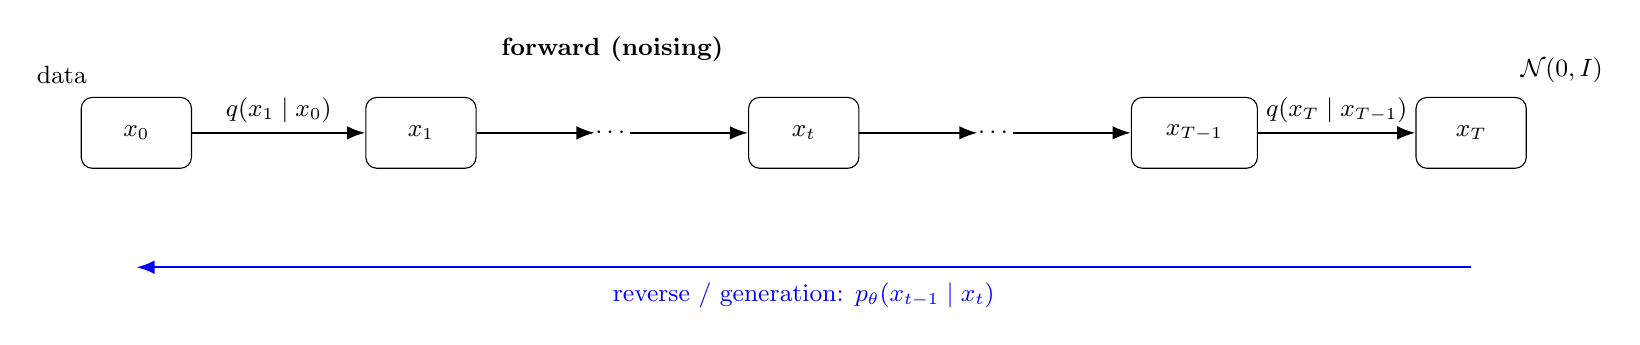
\begin{tikzpicture}[>=Latex, font=\small]
  % nodes
  \node[draw, rounded corners, minimum width=1.4cm, minimum height=0.9cm] (x0) {$x_0$};
  \node[draw, rounded corners, minimum width=1.4cm, minimum height=0.9cm, right=2.2cm of x0] (x1) {$x_1$};
  \node[inner sep=0pt, right=1.5cm of x1] (dots1) {$\cdots$};
  \node[draw, rounded corners, minimum width=1.4cm, minimum height=0.9cm, right=1.5cm of dots1] (xt) {$x_t$};
  \node[inner sep=0pt, right=1.5cm of xt] (dots2) {$\cdots$};
  \node[draw, rounded corners, minimum width=1.6cm, minimum height=0.9cm, right=1.5cm of dots2] (xTm1) {$x_{T-1}$};
  \node[draw, rounded corners, minimum width=1.4cm, minimum height=0.9cm, right=2.0cm of xTm1] (xT) {$x_T$};

  % forward (noising) arrows
  \draw[->, thick] (x0) -- node[above] {$q(x_1\mid x_0)$} (x1);
  \draw[->, thick] (x1) -- (dots1);
  \draw[->, thick] (dots1) -- (xt);
  \draw[->, thick] (xt) -- (dots2);
  \draw[->, thick] (dots2) -- (xTm1);
  \draw[->, thick] (xTm1) -- node[above] {$q(x_T\mid x_{T-1})$} (xT);

  % reverse (denoising) arrow (drawn below, avoid label overlaps)
  \coordinate (x0b) at ([yshift=-1.25cm]x0.south);
  \coordinate (xTb) at ([yshift=-1.25cm]xT.south);
  \draw[->, thick, blue] (xTb) -- node[below, yshift=-2pt] {reverse / generation: $p_\theta(x_{t-1}\mid x_t)$} (x0b);

  % labels
  \node[above=0.7cm of dots1] {\textbf{forward (noising)}};

  % endpoints annotations
  \node[above left=0.05cm and -0.2cm of x0] {$\text{data}$};
  \node[above right=0.05cm and -0.2cm of xT] {$\mathcal N(0,I)$};
\end{tikzpicture}
\end{document}


